\documentclass{article}
\usepackage{iclr2026_conference,times}

\usepackage{graphicx}
\usepackage{booktabs}
\usepackage{array}
\usepackage{amsmath}
\usepackage{amssymb}
\usepackage{listings}
\usepackage{xcolor}
\usepackage{hyperref}
\usepackage{url}

\definecolor{codebg}{HTML}{F6F7F9}
\definecolor{codekey}{HTML}{1F3B57}
\lstset{
  basicstyle=\ttfamily\scriptsize,
  backgroundcolor=\color{codebg},
  keywordstyle=\color{codekey}\bfseries,
  commentstyle=\color{gray}\itshape,
  frame=none, xleftmargin=6pt, framexleftmargin=6pt,
  aboveskip=5pt, belowskip=3pt, showstringspaces=false,
  columns=fullflexible, breaklines=true,
}

\title{Specifying What to Forget:\\A Domain-Agnostic Language\\for Behavioural Unlearning in RL}

\author{Anonymous authors\\Paper under double-blind review}

\newcommand{\fix}{\marginpar{FIX}}
\newcommand{\new}{\marginpar{NEW}}

% Uncomment for the camera-ready version only; submissions are anonymous.
% \iclrfinalcopy

\begin{document}
\maketitle

\begin{abstract}
Methods for removing a behaviour from a trained reinforcement-learning
policy take the behaviour as given. In practice it is fixed by a few lines
of environment-specific code that select which steps of a rollout to
forget, and the English description those lines implement often leaves
the selection open. We present \textsc{ForgetScenario}, a declarative
language for stating what to forget. Its only contact with a domain is a
\emph{feature view}, a map from observations, environment state and the
\texttt{info} dictionary to named, typed quantities that records how each
name was obtained, so a specification refers to quantities by name and
runs unchanged wherever a view supplies them. Over the view the language
provides conditions, regions, episode aggregates, quantifiers over agents
and a nestable temporal fragment with a formal semantics, together with a
validator that checks names, types and vacuity and a gate that admits a
learned view only above a stated held-out accuracy. We
instantiate the language in nine environments from five families and
evaluate it on fifteen behaviours, comparing each formalisation, step by step, with reference labels that language-model readers proposed from the
description alone and that we checked by hand. Six reproduce them
exactly. Agreement among the
readers locates each
remaining disagreement in the sentence or in the formalisation. A person
outside the author team labelled every step by hand, and these labels
agree with the reference at a median $\kappa$ of 0.95 and confirm four of
the five errors attributed to formalisations. A
controlled comparison shows that a description phrased as a goal is read
as its complement under every instruction we tried. Finally, choosing
which steps of an episode carry the label shifts the unlearned policy
beyond the effect of random label noise in a gridworld, and not in
continuous control.
\end{abstract}

\section{Introduction}

Suppose a deployed agent does something its operator wants stopped. It
routes through a region it should avoid, exploits a shortcut, or adopts a
gait that looks wrong. The unlearning literature offers a growing set of
procedures for removing such behaviour from a trained policy
\citep{bourtoule2021machine,cao2015towards,zhang2024npo}. Each of them
starts from a partition of experience into steps to forget and steps to
retain. How that partition is produced is rarely part of the
contribution.

In practice it is a predicate written by hand over whatever the
observation vector contains, applied to a rollout buffer, written
separately for each environment and seldom published with the method. It
also settles questions that the English description leaves open: where a
threshold lies, which steps of an episode count once the behaviour has
occurred, and which side of the sentence names the behaviour. Two papers
that report a forget rate on the same environment can therefore be
measuring different sets of steps.

We treat the specification as an artefact in its own right, with a
syntax, a semantics, a checker and an evaluation. Our contributions are
the following.

\begin{itemize}
\item \textbf{A language} (Section~\ref{sec:language}). A specification
never reads a policy's observation. It reads a feature view
$\Sigma:(o,\texttt{info},\texttt{env})\rightarrow\mathbb{R}^{n}$ whose
features carry names, types, ranges and a provenance recording how the
names were obtained. Over the view sits a grammar of conditions, regions,
derived features, episode aggregates, quantifiers over indexed agents and
a nestable temporal fragment, with a formal syntax and semantics
(Appendix~\ref{app:formal}). A validator checks names, types, ranges and
vacuity, and a learned view is admitted only above a stated held-out
fidelity.

\item \textbf{An evaluation protocol for specifications}
(Section~\ref{sec:eval}). Fidelity is measured step by step, with
chance-corrected agreement, against independent readings of the English
description, and the agreement among those readings decides whether a
disagreement belongs to the sentence or to the formalisation.

\item \textbf{Two measured consequences} (Sections~\ref{sec:polarity}
and~\ref{sec:drift}). Whether a description names the behaviour to remove
or the behaviour to keep decides which side readers label, whatever the
instruction. Which steps of an episode carry the label changes the
unlearned policy beyond the effect of random label noise in one of the two
domains we test.
\end{itemize}

\section{Related work}
\label{sec:related}

\paragraph{Machine unlearning.} Exact unlearning retrains without the
forgotten data \citep{bourtoule2021machine,cao2015towards}. Approximate
methods edit the trained model directly, and work on language models
supplies both benchmarks \citep{maini2024tofu} and objectives such as
negative preference optimisation \citep{zhang2024npo}. Throughout, the
forget set is given as a set of examples, so the question of how to
specify it does not arise.

\paragraph{Unlearning in reinforcement learning.}
\citet{ye2025reinforcement} unlearn an environment or one of its features.
\citet{gong2025trajdeleter} unlearn recorded trajectories from offline
agents, and \citet{zhang2025rule} use reinforcement learning as the
mechanism for unlearning in language models. In each case the target
arrives already delimited, as an environment, a set of episodes or a set
of queries. A behaviour is different. It has no extensional listing, every
policy realises it differently, and it changes under the unlearning update
itself, so it has to be described rather than enumerated. We are not
aware of prior work that treats that description as an object with a
syntax, a semantics and a measured fidelity.

\paragraph{Temporal logics and monitoring.} Linear temporal logic
\citep{pnueli1977temporal} underlies TLTL, whose quantitative semantics
turn a formula into a reward \citep{li2017tltl}, and reward machines expose
a reward function as an automaton over high-level events
\citep{icarte2018reward}. Monitors for signal temporal logic evaluate
formulas over finite recorded signals \citep{maler2004monitoring}, which is
also how our temporal fragment is used: a formula is checked at each
position of a finite episode. TLTL and reward machines specify behaviour
to be acquired, and all three assume a given map from states to the
propositions or signals a formula mentions. Our language makes that map
an explicit, typed object with a recorded provenance.

\paragraph{Constraints and shields.} Constrained policy optimisation
\citep{achiam2017cpo} and shielding \citep{alshiekh2018shielding} keep an
agent away from forbidden behaviour during training or execution. A
ForgetScenario can serve as their cost function or unsafe set, and the
reward-penalty baseline we run is an instance of that use.
Both lines of work take the forbidden set as given.

\paragraph{From natural language to formal specifications.} nl2spec
\citep{cosler2023nl2spec} and Lang2LTL \citep{liu2023lang2ltl} translate
English into temporal logic with language models and score a translation
against a reference formula. We compare at the level an unlearning method
consumes, the per-step labels a specification induces on trajectories,
and we also measure how far the English determines those labels at all.
Ambiguity in natural-language requirements is a long-standing concern of
requirements engineering \citep{berry2004ambiguity}, and the degree words
and polarity effects we measure are instances of its lexical and
pragmatic ambiguity.

\paragraph{Reward misspecification.} An objective that differs from the
intended one yields policies that exploit the difference
\citep{pan2022effects,skalse2022defining}. A misspecified forget target is
the mirror image. The method removes something, and the reported number
says that the intended behaviour is gone.

\paragraph{Language models as annotators.} Language models can match or
exceed crowd workers on text annotation \citep{gilardi2023chatgpt}, but
models of one family are not independent judges and tend to favour their
own outputs \citep{panickssery2024llm}. Our reference labels come from
such readers, and Section~\ref{sec:limitations} discusses what that does
and does not allow us to conclude. We report agreement as Cohen's
$\kappa$ \citep{cohen1960coefficient}.

\paragraph{Environments.} We use MiniGrid \citep{chevalier2023minigrid},
Gymnasium classic control and Box2D \citep{towers2024gymnasium}, MuJoCo
\citep{todorov2012mujoco} and level-based foraging
\citep{papoudakis2021benchmarking}.

\section{The language}
\label{sec:language}

\subsection{Feature views}
\label{sec:views}

The observation is frequently the wrong place to look. A MiniGrid agent
may observe a $7\times7\times3$ egocentric image in which no index means
\texttt{agent\_x}, and Gymnasium's MuJoCo wrappers drop the root $x$
coordinate so that policies stay translation invariant. A language that
reads observations directly inherits both problems.

A view is a map
$\Sigma:(o,\texttt{info},\texttt{env})\rightarrow\mathbb{R}^{n}$ together
with the names, types and ranges of its $n$ features. Because $\Sigma$
may read the \texttt{info} dictionary and the environment object, a
scenario can be written over quantities the agent never observes. Views
resolve through a cascade of tiers, and each view records how it was
obtained:

\begin{center}
\begin{tabular}{@{}lll@{}}
\toprule
Provenance & Tier & How the names were obtained \\
\midrule
\texttt{auto:<domain>} & environment & introspected from the environment \\
\texttt{declared:table} & table & hand-registered name table \\
\texttt{auto:info\_dict} & generic & scalar keys read from \texttt{info} \\
\texttt{declared:identity} & fallback & anonymous \texttt{dim\_0, dim\_1, \dots} \\
\texttt{learned:<kind>} & learned & fitted from data, with a fidelity score \\
\bottomrule
\end{tabular}
\end{center}

Provenance makes portability checkable, and it exposes a failure that
integer indices hide. Under a hand-written HalfCheetah table
\texttt{rooty} is index 1, while under \texttt{auto:mujoco}, which indexes
$q_{\text{pos}}\mathbin\Vert q_{\text{vel}}$ including the dropped root
coordinate, it is index 2. A scenario written as \texttt{dim: rooty} is
correct under both, and one written as \texttt{dim: 1} under only one.
Appendix~\ref{app:views} lists the view of every environment in the
corpus.

\subsection{Scenarios}
\label{sec:grammar}

A scenario is a YAML document checked against a JSON Schema. Its
state-level core is a group expression: a conjunction of conditions on
named features, boolean combinations of groups, and region shorthands
(boxes, their complements, ellipsoids and polygons). \texttt{derived}
defines new features by arithmetic over a whitelist of functions.
\texttt{aggregates} reduce an episode to scalars such as sums, extrema and
distinct counts. \texttt{families} index repeated blocks of features, such
as one block per agent, and a derived feature can quantify over their
members with \texttt{min}, \texttt{max}, \texttt{any} or \texttt{all}, so
that the scenario does not depend on team size. A temporal formula
combines group expressions with \texttt{not}, \texttt{and}, \texttt{or},
\texttt{next}, \texttt{previous}, \texttt{eventually}, \texttt{always},
\texttt{until}, \texttt{consecutive} and \texttt{then\_within}, nested to
any depth and evaluated at a position of a finite episode.

Two fields turn a predicate into training labels. \texttt{match\_mode}
decides which episodes are selected: an episode is selected when any step
matches, when all steps match, when the fraction of matching steps reaches
a threshold, when a condition on its aggregates holds, or when a temporal
formula holds at its first step. \texttt{applies\_to} decides which steps
carry the label. Under \texttt{matching\_steps} a step is labelled when
the state predicate, or the temporal formula, holds at that step. Under
\texttt{whole\_trajectory} every step of a selected episode is labelled.
Selection is made per episode, so a rollout buffer that concatenates
several episodes is first split at episode boundaries.
Appendix~\ref{app:formal} gives the grammar and the labelling function
formally. Figure~\ref{fig:examples} shows three formalisations from the
corpus, one quantifying over agents, one built from episode aggregates and
one temporal, and Appendix~\ref{app:gallery} lists every formalisation
next to its description.

\begin{figure}[t]
\centering
\begin{minipage}[t]{0.53\textwidth}
{\footnotesize\textbf{(a)} Foraging-8x8-3p-2f-v3\\\textit{``Stop the agents from bunching up instead of spreading out to forage.''}}
\begin{lstlisting}[language=,aboveskip=2pt,belowskip=2pt,basicstyle=\ttfamily\fontsize{6.5}{7.6}\selectfont]
match_mode: proportion
match_threshold: 0.2
applies_to: matching_steps
families: {agent: "p{i}_"}
derived:
  closest_pair:
    over: agent
    arity: 2
    reduce: min
    expr: "abs(a_row - b_row) + abs(a_col - b_col)"
groups:
- name: agents_crowded
  conditions:
  - {dim: closest_pair, op: "<", value: 2}
\end{lstlisting}
\end{minipage}
\hfill
\begin{minipage}[t]{0.45\textwidth}
{\footnotesize\textbf{(b)} MiniGrid-FourRooms-v0\\\textit{``Stop revisiting cells the agent has already been to in this episode.''}}
\begin{lstlisting}[language=,aboveskip=2pt,belowskip=2pt,basicstyle=\ttfamily\fontsize{6.5}{7.6}\selectfont]
match_mode: trajectory
applies_to: whole_trajectory
aggregates:
  cells_visited:
    op: count_distinct
    of: [agent_x, agent_y]
  path_length: {op: count}
derived:
  revisits: "path_length - cells_visited"
groups:
- name: backtracks
  conditions:
  - {dim: revisits, op: ">", value: 4}
\end{lstlisting}
\end{minipage}
\\[6pt]
\begin{minipage}[t]{0.9\textwidth}
{\footnotesize\textbf{(c)} MiniGrid-FourRooms-v0\\\textit{``Stop the reflex of turning left at or immediately after entering the bottom-right room (within one step of crossing the boundary).''}}
\begin{lstlisting}[language=,aboveskip=2pt,belowskip=2pt,basicstyle=\ttfamily\fontsize{7.0}{8.1}\selectfont]
match_mode: temporal
applies_to: matching_steps
temporal:
  and:
  - conditions:
    - {dim: 0, dim_name: agent_x, op: ">", value: 9.5, target: state}
    - {dim: 1, dim_name: agent_y, op: ">", value: 9.5, target: state}
    - {dim: 0, dim_name: turn_left, op: "==", value: 0, target: action}
  - or:
    - previous:
        conditions:
        - {dim: 0, dim_name: agent_x, op: "<", value: 9.5, target: state}
    - previous:
        previous:
          conditions:
          - {dim: 0, dim_name: agent_x, op: "<", value: 9.5, target: state}
\end{lstlisting}
\end{minipage}
\caption{Three formalisations from the corpus, each under the English description it was written for. \textbf{(a)} A derived feature that quantifies over the members of a family of agents, so one file serves any team size. \textbf{(b)} Two episode aggregates combined by arithmetic. \textbf{(c)} A nested temporal formula. The agent turns left inside the room, and was outside it one or two steps earlier, so the label falls on the turn at the crossing and not on later turns. Features are named, as in (a) and (b), or indexed with a \texttt{dim\_name} that the validator checks against the bound view, as in (c). Comments and the \texttt{name} and \texttt{description} fields are omitted, and (c) also omits a state-level group that serves evaluation only. Appendix~\ref{app:gallery} lists every formalisation.}
\label{fig:examples}
\end{figure}


\subsection{Validation}
\label{sec:validation}

The validator works in three stages. The schema stage checks structure.
The view stage resolves every feature name against the bound view and
rejects unknown names, contradictory conditions and aggregates outside a
trajectory-level match mode. It warns when a comparison does not suit a
feature's type, such as ordering a categorical feature, and when a
threshold lies outside a feature's declared range, so that a condition can
never hold or always holds. When rollouts are supplied, the empirical
stage rejects a specification that labels no step or every step. Further
warnings flag constructions whose labels are probably not what the author
meant, and Appendix~\ref{app:validator} shows the validator's messages on a
set of faulty scenarios.
An existential temporal operator at the top level of a
\texttt{matching\_steps} formula, for example, labels every step up to the
last witness rather than the witness itself.

These checks establish that a specification is well formed and not
vacuous. They do not establish that it means what its description says. We
stress-tested them with two open code models, Qwen2.5-Coder 7B and 32B,
writing scenarios from the thirteen descriptions the grammar states exactly
(Appendix~\ref{app:authoring}). The validator accepted 85\% and 77\% of
their scenarios. On the four FourRooms entries, where it also ran the
empirical stage, each model had two scenarios accepted and none was
vacuous. Yet all four labelled different steps from our formalisations,
with a Jaccard similarity between 0.00 and 0.18. Passing every check is
easy and says little about meaning. We therefore make no claim that models
can author scenarios, and we measure fidelity separately
(Section~\ref{sec:eval}).

One further check reads the description rather than the specification. A
behaviour description must name the behaviour to remove, and a lint run
over the corpus flags a description that does not open with a prohibition
such as \emph{stop}, \emph{never} or \emph{avoid}. Section~\ref{sec:polarity}
measures why this matters.

\subsection{Learned views}
\label{sec:learned}

Every tier above rests on someone already knowing what the features mean.
A raw pixel observation offers no such foothold. A probe closes the gap:
it is fitted from raw observations to the semantic features a scenario
needs, and its predictions are exposed as a view. A fitted view can be
wrong, and a wrong view is worse than a missing one, because every
scenario written against it inherits the error silently. The probe is
therefore fitted on one split and scored on another, per feature, and the
view carries the score of its weakest feature, since a scenario may
depend on any of them. A view scoring below a stated threshold (0.9 here)
is refused.

Both outcomes occur (Figure~\ref{fig:probe}). From a full-grid render of
FourRooms, position is recovered with exact-match accuracy 0.947 and
0.959, and a spatial scenario runs unchanged on pixels, agreeing with the
ground-truth labels on 400 of 400 steps. From the egocentric observation
the same procedure scores 0.06 and the view is refused. That is the
correct outcome, because a partially observed view does not determine
absolute position.

\begin{figure}[t]
\centering
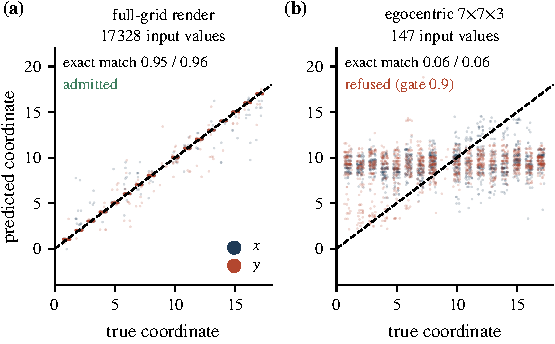
\includegraphics[width=0.80\textwidth]{figures/fig_probe.pdf}
\caption{Held-out probe predictions against ground truth on
MiniGrid-FourRooms, 4769 samples, with $x$ and $y$ jittered horizontally
for legibility. The dashed line is $y=x$. \textbf{(a)} The full-grid
render determines the agent's position and the probe recovers it, so the
view is admitted. \textbf{(b)} The egocentric observation does not
determine it. The probe collapses onto the mean and is refused. Scores are
exact match after rounding, the criterion the gate applies to an ordinal
feature.}
\label{fig:probe}
\end{figure}

\section{Evaluating specifications}
\label{sec:eval}

\subsection{The behaviours}
\label{sec:corpus}

The evaluation covers fifteen behaviours over nine environments in five
families, each stated in one English sentence of the kind an operator
would write when asking for a behaviour to be removed. Thirteen are
formalised exactly. Two are formalised approximately (\emph{partial}),
because the grammar cannot count a repeated pattern of cells or measure
the distance to a failure that did not happen, and each records the
approximation it uses. Appendix~\ref{app:corpus} lists them.

\subsection{Reference labels}
\label{sec:readers}

Fidelity needs a reference that owes nothing to the formalisation it
judges. We built ours in two stages over the recorded rollouts of the
fifteen entries, 6272 steps in all and between 77 and 1600 per entry. In
the first stage, language-model readers proposed a label for every step
from the description alone. Each reader was an instance of Claude Opus~5
that we started from a fresh context under prompts we wrote. It saw the
English sentence and a table of per-step feature values and nothing
else: no scenario file, no other reader's labels and no result. Where the
sentence left a threshold or a time span open, the reader had to choose
one and state it before labelling, so every choice that a sentence leaves
to its reader is on record. Two or three readers read each entry, and
their common labels, or the per-step majority where they differed,
formed the proposal. In the second stage we checked every proposed label
by hand against the description and the feature values. The first stage
keeps the reading independent of the formalisation, and the second makes
a person answerable for every label. The reference labels are ours. Our
check confirmed every proposal, so the reference coincides with the
readers' labels and the analyses of reader agreement below apply to it
directly. Appendix~\ref{app:readers} gives every round of readers, our
prompts in full and the proposals we discarded.

The first round used a neutral instruction, to decide for every step
whether the described behaviour is occurring. One of its three readers
marked the complementary set on all four of its entries, and its labels
were aligned in polarity to those of the other two readers, never to the
formalisation, before the majority was taken. Later rounds stated that the
sentence names a behaviour to be stopped and asked for the steps where it
happens. Section~\ref{sec:polarity} measures what that instruction does.

\subsection{Fidelity}
\label{sec:fidelity}

Fidelity is the per-step agreement between the labels a formalisation
produces and the reference. We report Cohen's $\kappa$, because Jaccard
similarity ignores agreement on unlabelled steps and loses resolution on
rare behaviours (Appendix~\ref{app:corpus} gives both, with precision and
recall). Mean $\kappa$ over the fifteen entries is 0.555 and the
distribution is bimodal (Figure~\ref{fig:fidelity}). Six formalisations
reproduce the reference exactly. Five of their descriptions fix a
criterion: a half of the track, a quadrant of the room, a turn within one
step of entering a room. The sixth asks for no ``steep tilt'', and its
three readers and its formalisation all chose the same threshold of
0.2~rad. Four entries score below 0.12.

A low score does not say by itself whether the formalisation or the
sentence is at fault. Agreement among the readers decides it. On eleven
of the fifteen entries the readers labelled exactly the same steps, so for
them the sentence determined a set of steps, and a formalisation that
differs from that set is the outlier. Five formalisations are in this
position. Four of them label whole episodes, where the readers label
only the steps of the act itself: holding a key that is never used,
revisiting cells, pacing between two cells, and turning a somersault.
Their recall is 1.00 and their precision at most 0.43. None of the four
narrower readings can be written with the views and operators we have.
For the key it needs a feature recording whether the door is open, which
the MiniGrid view does not expose, and the toggle action is no substitute
because a toggle need not open anything. For the other three, marking a single step as a
revisit, an oscillation or part of a rotation means relating it to values
at earlier steps, which the fragment cannot do. Their formalisations settle for an episode-level reading, and the
readers show what that reading leaves out. The fifth formalisation
approximates a near miss through the lander's tilt.

On the remaining four entries the readers disagree with one another
($\kappa$ from 0.44 to 0.93), and there the sentence is underdetermined.
Three rest on a degree word: ``bunching up'', ``idles nearby'' and ``past
the angle that precedes a face-first fall''. The readers chose
different thresholds, and the formalisation is one more such choice. The
fourth, ``stop using the doorway between the bottom-right and top-right
rooms'', is underdetermined in time rather than in degree. Its three
readers found the same seven doorway steps in the same six episodes and
then labelled 12, 18 and 29 steps, because the sentence says where the act
happens and not how long it lasts. Its formalisation also fails for a
reason of its own. It places the doorway at a fixed cell, while the
environment moves the doorways at every reset, so it labels four steps
that no reader chose ($\kappa=0.00$). The validator accepts it, since it
is well typed and labels some steps but not all.

Every reader is a language model, and readers of one family can agree on a
reading that a person would not take. A person outside the author team
therefore labelled all
6272 steps by hand, in a tool that shows the description, the features
and the actions but no labels or formalisations. These labels agree with
the reference at a median $\kappa$ of 0.95, mean 0.79, and match it
exactly on six entries (crosses in Figure~\ref{fig:fidelity}). On the four
entries whose formalisations label whole episodes the person sides with
the readers, at $\kappa$ from 0.92 to 1.00 against the reference and at
most 0.54 against the formalisation. Where the readers disagree, the
person makes one more choice, and for the forward fall it is the
formalisation's threshold ($\kappa=1.00$ against it). Two departures fall
where the readers were unanimous. The person put a steep tilt at 15
degrees, where every reader chose 0.2~rad ($\kappa=0.83$). For the near
miss, the readers marked the last 12 to 19 steps before each impact. Every
recorded episode, however, ends with the lander striking the ground or
leaving the screen, so no landing narrowly avoided a crash, and the person
labelled no step. Unanimity among readers of one family, and our check of
their labels, did not settle these two readings.

\begin{figure}[t]
\centering
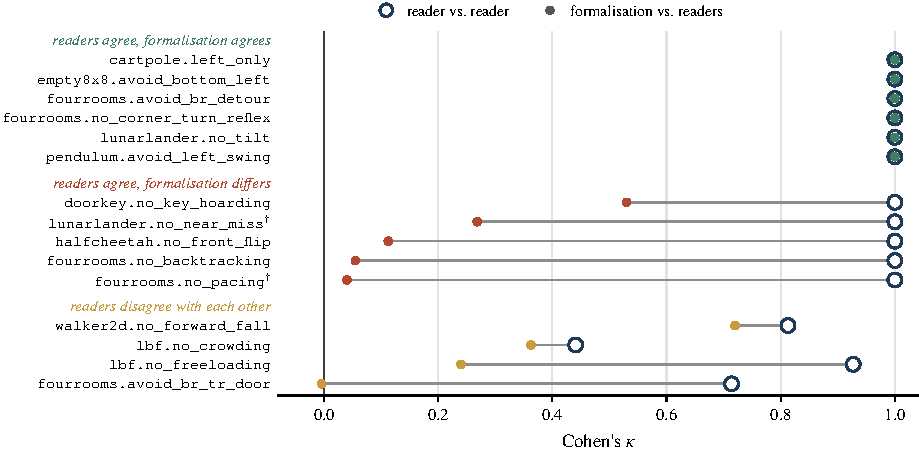
\includegraphics[width=\textwidth]{figures/fig_fidelity.pdf}
\caption{Agreement on the fifteen labelled entries. Open circles:
agreement between readers of the same description (mean pairwise
$\kappa$). Dots: agreement between the formalisation and the reference
labels. Crosses: agreement between one person's labels, made by hand,
and the reference labels. Entries are grouped by where the disagreement
lies. Where the
readers agree with each other, a low dot points at the formalisation.
Where they do not, the sentence leaves the labels open. $^{\dagger}$Partial
entries, formalised approximately.}
\label{fig:fidelity}
\end{figure}

\subsection{Polarity}
\label{sec:polarity}

A description can name the behaviour to keep rather than the one to
remove. Three descriptions in the corpus had such a goal wording, for
example ``Balance the pole only while the cart stays on the left half of
the track''. Readers given such a sentence label the
behaviour it names, which is the behaviour to keep, and so mark the exact
complement of the formalisation. Table~\ref{tab:polarity} separates the
sentence from the instruction. Their goal wording was read under
neutral instructions and under the strict one,
which states that the sentence names a behaviour to be stopped, and it
was read as its complement in all 13 reader--entry pairs. For the nine
pairs whose labels were kept, $\kappa$ against the formalisation lies
between $-0.49$ and $-1.00$, and between 0.98 and 1.00 after flipping.
Prohibitions, among them the rewrites of the same three behaviours
(``Stop balancing the pole while the cart is on the right half of the
track''), were read correctly in all 23 pairs under the strict
instruction. Under a neutral instruction, one of three readers inverted
all four prohibitions it saw and the other two inverted none.

\begin{table}[t]
\centering
\caption{Reader--entry pairs whose labels mark the complement of the
formalisation, by the voice of the description and the instruction given
to the reader. The strict instruction states that the sentence names a
behaviour to be stopped.}
\label{tab:polarity}
\begin{tabular}{@{}lcc@{}}
\toprule
Description & Neutral instruction & Strict instruction \\
\midrule
Goal (names the behaviour to keep) & 7 of 7 & 6 of 6 \\
Prohibition (names the behaviour to remove) & 4 of 12 & 0 of 23 \\
\bottomrule
\end{tabular}
\end{table}

The defect lies in the sentence. Stating the convention in the
instruction removes readers' errors on prohibitions but not on goals, and
the readers that inverted goal-voice sentences under that instruction did
what it said. They took the sentence to name the behaviour to stop. A
description should therefore carry its own polarity, which is what the
lint checks. On the eighteen descriptions that readers have labelled, it
flags the three that every reader inverted and none of the other fifteen.
Every current description passes (Appendix~\ref{app:lint}).

\section{Label scope and the unlearned policy}
\label{sec:drift}

The field \texttt{applies\_to} exists because ``stop routing through the
bottom-right room'' does not say whether the label belongs to the steps in
the room or to every step of an episode that routes through it. We test
whether that choice changes the outcome of unlearning. Two scenario files
that differ only in this field were used to unlearn from the same
baseline checkpoints in FourRooms and CartPole, fifteen seeds per arm,
with a reward penalty of $\lambda=0.1$ on labelled steps
(Appendix~\ref{app:methods}). The pipeline is deterministic given a
configuration and a seed, so two runs on one seed differ only through
their labels. On rollouts of the baselines, the two readings label 20\% of
steps differently in FourRooms and 33\% in CartPole.

Training amplifies any change to the labels, so the size of a difference
between two policies means little without a reference. We therefore add
control runs that flip a random 1\% of labels, and in FourRooms also
10\%, using a random generator separate from action sampling and
environment resets. Every arm is compared with the \texttt{matching\_steps}
run on the same seed, by the fraction of states, drawn from the baseline,
on which the two policies choose the same action, and by the shift in
forget-region occupancy after the last update.

\begin{figure}[t]
\centering
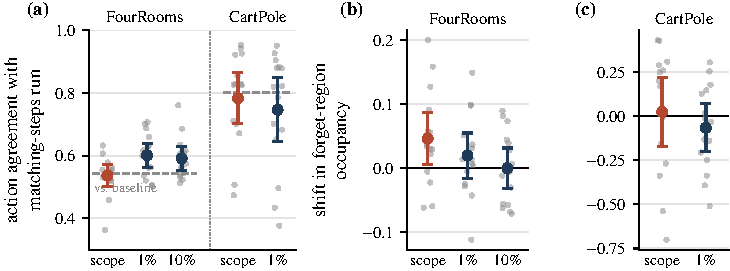
\includegraphics[width=\textwidth]{figures/fig_drift.pdf}
\caption{Each arm against the \texttt{matching\_steps} run on the same
seed. \emph{scope}: the \texttt{whole\_trajectory} reading. \emph{1\%},
\emph{10\%}: the \texttt{matching\_steps} reading with that fraction of
labels flipped at random. Small dots are seeds, and bars are 95\%
intervals over fifteen seeds. \textbf{(a)} Fraction of shared states on
which the two policies choose the same action. The dashed line is the
agreement of the \texttt{matching\_steps} run with its baseline.
\textbf{(b, c)} Shift in final forget-region occupancy, on separate scales
for the two domains.}
\label{fig:drift}
\end{figure}

Random flips alone move the policy about as far as unlearning moved it
from its baseline (Figure~\ref{fig:drift}a). With 1\% of labels flipped,
FourRooms policies agree with the unperturbed run on 60\% of states,
against 54\% between that run and its baseline, and flipping 10\% of
labels gives 59\%. Agreement between two runs is therefore no
evidence by itself that a specification matters. Against this floor the
two domains differ. In FourRooms the other reading moves the policy
further than either noise level (agreement 0.54, $p<0.01$, and lower on
11 of 15 seeds in each comparison), and it raises forget-region occupancy
by 0.046 ($p=0.03$) where the noise runs shift it by 0.019 and 0.000
($p=0.26$ and $0.98$). Compared directly with the 10\% control, the
occupancy shift is larger by 0.046 ($p=0.06$). In CartPole the other reading cannot
be told apart from 1\% noise on either measure. On the baselines'
rollouts the \texttt{whole\_trajectory} reading labels 91\% of CartPole
steps, so the penalty it adds is close to a constant and carries little
information about where the cart is.

\section{Limitations}
\label{sec:limitations}

\paragraph{Readers.} All 22 readers are language models of one family:
twenty instances of Claude Opus~5, which proposed every reference label,
and two of Claude Opus~5.5 in the polarity experiment. They are not
independent in
the way a panel of people is. Models of one family share priors and
favour their own outputs \citep{panickssery2024llm}, so unanimity among
them can reflect a shared bias. One person's labels show this on two
entries, the steep tilt and the near miss, while supporting the
attributions of Section~\ref{sec:fidelity} on the others. Our check of
every label by hand guards against a reader's mistake but not against a
reading we share with the readers, as the near miss shows. An independent
annotator removes the dependence on one model family for the fidelity
diagnosis, but one person is not a panel, and the polarity effect was
measured with models only. The
instructions also differed between rounds. Later rounds named the choice
of span for behaviours that extend in time, which may have influenced the
spans readers chose (Appendix~\ref{app:readers}).

\paragraph{Scale.} The corpus has fifteen behaviours, labelled on
77 to 1600 steps each. The label-scope experiment varies one construct on one
scenario per domain, with one unlearning method and fifteen seeds per arm,
and its effect appears in one of the two domains. The method comparison
in Appendix~\ref{app:comparison} uses five seeds, and no difference in it
survives correction for multiple comparisons.

\paragraph{Authorship.} We wrote the corpus, its formalisations and the
readers' prompts, so the choice of behaviours reflects our judgement of
what an operator would want removed.

\section{Conclusion}

Unlearning in reinforcement learning cannot be separated from the
question of what is to be unlearned. We have argued that the
specification should be built like any other component of the method:
typed, checked, connected to the domain through an explicit interface,
and evaluated for what it can and cannot say. Measured that way, the
specifications in our corpus fail in identifiable places. Several
formalisations label whole episodes where readers, and a person labelling
by hand, label only the act, and the language cannot yet state the
narrower reading. Some
descriptions do not determine a set of steps at all, and a description in
the wrong voice is read as its own complement. The first is a measured
limit of the grammar, the second a property of the English that no
formalisation can repair, and the third is caught by a lint. Each becomes
visible only because the specification is an explicit object that can be
compared with an independent reading of its description.

\subsubsection*{Reproducibility statement}

All environments are publicly available. The training pipeline is
deterministic given a configuration and a seed.
Appendix~\ref{app:methods} lists the training and unlearning settings and
Appendix~\ref{app:readers} the reader prompts. We will release the
language, the validator, the corpus with its formalisations, the reference
labels with every reader prompt, one person's labels of every step, and
the scripts that produce each number
and figure in the paper.

\bibliography{references}
\bibliographystyle{iclr2026_conference}

\appendix

\section{Syntax and semantics}
\label{app:formal}

\paragraph{Syntax.} The concrete syntax is YAML validated by a JSON
Schema. Abstracting from it, a scenario is generated by the following
grammar, where $f$ ranges over feature names (including derived ones),
$c$ over numeric constants, $k,w$ over positive integers and $\theta$ over
$[0,1]$.
\begin{align*}
\mathit{scenario} &::= \mathit{decls}\;\; \texttt{match\_mode}\;m\;\;[\texttt{match\_threshold}\;\theta]\\
&\quad\;\;\texttt{applies\_to}\;s\;\;(\mathit{groups}\mid\varphi)\\
m &::= \texttt{any\_step}\mid\texttt{all\_steps}\mid\texttt{proportion}\\
&\quad\;\;\mid\texttt{top\_percentile}\mid\texttt{trajectory}\mid\texttt{temporal}\\
s &::= \texttt{matching\_steps}\mid\texttt{whole\_trajectory}\\
\mathit{groups} &::= G_1,\dots,G_m \qquad\text{(disjunction)}\\
G &::= C_1\wedge\dots\wedge C_k \mid \texttt{all\_of}(G,\dots)\mid\texttt{any\_of}(G,\dots)\\
&\quad\;\;\mid\texttt{not}(G)\mid R\mid\texttt{\$ref}\;\mathit{name}\\
C &::= f\;\mathit{op}\;c \;\;[\texttt{target}\;t] \mid \texttt{action\_sequence}(a_1,\dots,a_k)\\
\mathit{op} &::= \;>\;\mid\;\ge\;\mid\;<\;\mid\;\le\;\mid\;=\;\mid\;\ne\;\mid\;\texttt{abs>}\;\mid\;\texttt{abs>=}\;\mid\;\texttt{abs<}\;\mid\;\texttt{abs<=}\\
t &::= \texttt{state}\mid\texttt{action}\mid\texttt{reward}\mid\texttt{return}\mid\texttt{length}\\
R &::= \texttt{box}(\vec f,\vec{lo},\vec{hi})\mid\texttt{complement\_of\_box}(\vec f,\vec{lo},\vec{hi})\\
&\quad\;\;\mid\texttt{ellipsoid}(\vec f,\vec c,\vec r)\mid\texttt{polygon}(f_1,f_2,\vec v)\\
\varphi &::= G\mid\neg\varphi\mid\varphi\wedge\dots\wedge\varphi\mid\varphi\vee\dots\vee\varphi\mid\mathsf{X}\varphi\mid\mathsf{Y}\varphi\\
&\quad\;\;\mid\mathsf{F}\varphi\mid\mathsf{G}\varphi\mid\varphi\,\mathsf{U}\,\varphi\mid\mathsf{C}_k\varphi\mid\varphi\,\mathsf{T}_w\,\varphi
\end{align*}
Here $\mathsf{X}$, $\mathsf{Y}$, $\mathsf{F}$, $\mathsf{G}$, $\mathsf{U}$,
$\mathsf{C}_k$ and $\mathsf{T}_w$ are \texttt{next}, \texttt{previous},
\texttt{eventually}, \texttt{always}, \texttt{until}, \texttt{consecutive}
and \texttt{then\_within}. The declarations $\mathit{decls}$ are
\begin{itemize}
\item \texttt{defines}: named group expressions, referenced with \texttt{\$ref};
\item \texttt{derived}: $f := e$, where $e$ is an arithmetic expression
over feature names and constants with $+,-,\times,/$ and the functions
\texttt{abs}, \texttt{min}, \texttt{max}, \texttt{sqrt}, \texttt{hypot},
\texttt{floor}, \texttt{ceil} and \texttt{sign}, or a quantified
expression $f := \rho_{\,b_1,\dots,b_a\in F}\,e$ over the members of a
family $F$ with arity $a\le 8$ and reduction
$\rho\in\{\min,\max,\Sigma,\text{mean},\text{count},\exists,\forall\}$;
\item \texttt{aggregates}: $g := \alpha(f)$ with
$\alpha\in\{$sum, mean, min, max, std, range, first, last, abs\_sum,
n\_distinct, count, count\_distinct$\}$, optionally restricted to the
steps satisfying a group;
\item \texttt{families}: a name template containing \texttt{\{i\}}, whose
members are discovered in the bound view.
\end{itemize}

\paragraph{Typing.} Each feature of the bound view has a type in
$\{$continuous, ordinal, categorical, boolean$\}$ and an optional range.
A condition must name a feature of the view or a declared derived feature
or aggregate, and an aggregate may be used only under
\texttt{match\_mode: trajectory}. Violations are errors. An order
comparison on a categorical or boolean feature, and a constant outside a
feature's range, which makes a condition constant, produce warnings.

\paragraph{Semantics.} Let an episode be $\tau=(x_t,a_t,r_t)_{t=0}^{n-1}$,
where $x_t=\Sigma(o_t,\texttt{info}_t,\texttt{env}_t)$ is extended with
the derived features. A condition $f\,\mathit{op}\,c$ holds at $t$ when
$\mathit{op}(x_t[f],c)$ holds, reading $a_t$ or $r_t$ instead of $x_t$
for the targets \texttt{action} and \texttt{reward}. A conjunction holds
when all its conditions do, combinators are interpreted as usual, and a
box holds when $lo_j\le x_t[f_j]\le hi_j$ for every listed feature. A
list of groups holds when one of them does. We write $t\models G$.

A temporal formula is evaluated at a position $0\le t<n$ and is false at
any position outside the episode:
\begin{align*}
t\models\mathsf{X}\varphi &\iff t+1\models\varphi\\
t\models\mathsf{Y}\varphi &\iff t-1\models\varphi\\
t\models\mathsf{F}\varphi &\iff \exists u\in[t,n).\;u\models\varphi\\
t\models\mathsf{G}\varphi &\iff \forall u\in[t,n).\;u\models\varphi\\
t\models\varphi\,\mathsf{U}\,\psi &\iff \exists u\in[t,n).\;u\models\psi\wedge\forall v\in[t,u).\;v\models\varphi\\
t\models\mathsf{C}_k\varphi &\iff \exists u\in[t,n-k].\;\forall i<k.\;u+i\models\varphi\\
t\models\varphi\,\mathsf{T}_w\,\psi &\iff \exists u\ge t.\;u\models\varphi\wedge\exists v\in(u,\min(u+w,n-1)].\;v\models\psi
\end{align*}
with $\neg$, $\wedge$ and $\vee$ interpreted pointwise. $\mathsf{U}$ is
the strong until. $\mathsf{C}_k$ and $\mathsf{T}_w$ are existential over
later positions.

\paragraph{Selection and labels.} An episode is selected,
$\tau\in\mathrm{Sel}$, under
\begin{center}
\begin{tabular}{@{}ll@{}}
\texttt{any\_step} & $\exists t.\;t\models G$ \\
\texttt{all\_steps} & $\forall t.\;t\models G$ \\
\texttt{proportion} & $|\{t: t\models G\}|/n\ge\theta$ \\
\texttt{trajectory} & $G$ holds of the episode's aggregates, \texttt{return} and \texttt{length} \\
\texttt{temporal} & $0\models\varphi$ \\
\texttt{top\_percentile} & $\tau$ is in the top $\theta$ fraction of the batch by return or length
\end{tabular}
\end{center}
Only \texttt{top\_percentile} depends on other episodes. The label of step
$t$ is
\[
L(\tau)_t=\begin{cases}
[\tau\in\mathrm{Sel}] & \texttt{applies\_to}=\texttt{whole\_trajectory},\\
[t\models\varphi] & \texttt{applies\_to}=\texttt{matching\_steps},\ \texttt{match\_mode}=\texttt{temporal},\\
[t\models G] & \texttt{applies\_to}=\texttt{matching\_steps},\ \text{otherwise}.
\end{cases}
\]
Under \texttt{matching\_steps} a non-temporal match mode therefore
affects which episodes are reported as matching but not which steps are
labelled. A rollout buffer $B$ is split at its episode boundaries,
$B=\tau^{1}\cdots\tau^{m}$, and labelled episode by episode,
$L(B)=L(\tau^{1})\cdots L(\tau^{m})$. With \texttt{matching\_steps}, a
top-level $\mathsf{F}\varphi$ labels every step up to the last position
at which $\varphi$ holds, and the validator warns about this
construction.

\section{Feature views}
\label{app:views}

Table~\ref{tab:views} lists the view each environment of the corpus resolves to, with its provenance and the names a scenario may use. The MiniGrid and MuJoCo views are introspected from the environment, the level-based foraging view from its \texttt{info} and environment state, and the classic-control and Box2D views come from hand-registered tables. Feature types are boolean, categorical, continuous, ordinal.

\begin{table}[h]\centering\footnotesize
\caption{Resolved feature views. MiniGrid's three environments share one view.}
\label{tab:views}
\begin{tabular}{@{}>{\raggedright\arraybackslash}p{2.5cm}lr>{\raggedright\arraybackslash}p{6.4cm}@{}}\toprule
Environment & Provenance & $n$ & Features \\ \midrule
CartPole-v1 & \texttt{declared:table} & 4 & \texttt{cart\_position}, \texttt{cart\_velocity}, \texttt{pole\_angle}, \texttt{pole\_angular\_velocity} \\
Foraging-8x8-3p-2f-v3 & \texttt{auto:lbf} & 14 & \texttt{p0\_row}, \texttt{p0\_col}, \texttt{p0\_level}, \texttt{p0\_score}, \texttt{p1\_row}, \texttt{p1\_col}, \texttt{p1\_level}, \texttt{p1\_score}, \texttt{p2\_row}, \texttt{p2\_col}, \texttt{p2\_level}, \texttt{p2\_score}, \texttt{n\_food}, \texttt{food\_level\_total} \\
HalfCheetah-v5 & \texttt{auto:mujoco} & 18 & \texttt{rootx}, \texttt{rootz}, \texttt{rooty}, \texttt{bthigh}, \texttt{bshin}, \texttt{bfoot}, \texttt{fthigh}, \texttt{fshin}, \texttt{ffoot}, \texttt{v\_rootx}, \texttt{v\_rootz}, \texttt{v\_rooty}, \texttt{v\_bthigh}, \texttt{v\_bshin}, \texttt{v\_bfoot}, \texttt{v\_fthigh}, \texttt{v\_fshin}, \texttt{v\_ffoot} \\
LunarLander-v3 & \texttt{declared:table} & 8 & \texttt{x}, \texttt{y}, \texttt{vx}, \texttt{vy}, \texttt{angle}, \texttt{angular\_velocity}, \texttt{left\_leg\_contact}, \texttt{right\_leg\_contact} \\
MiniGrid: Empty, FourRooms, DoorKey & \texttt{auto:minigrid} & 5 & \texttt{agent\_x}, \texttt{agent\_y}, \texttt{direction}, \texttt{carrying\_key}, \texttt{carrying\_any} \\
Pendulum-v1 & \texttt{declared:table} & 3 & \texttt{cos\_theta}, \texttt{sin\_theta}, \texttt{theta\_dot} \\
Walker2d-v5 & \texttt{auto:mujoco} & 18 & \texttt{rootx}, \texttt{rootz}, \texttt{rooty}, \texttt{thigh\_joint}, \texttt{leg\_joint}, \texttt{foot\_joint}, \texttt{thigh\_left\_joint}, \texttt{leg\_left\_joint}, \texttt{foot\_left\_joint}, \texttt{v\_rootx}, \texttt{v\_rootz}, \texttt{v\_rooty}, \texttt{v\_thigh\_joint}, \texttt{v\_leg\_joint}, \texttt{v\_foot\_joint}, \texttt{v\_thigh\_left\_joint}, \texttt{v\_leg\_left\_joint}, \texttt{v\_foot\_left\_joint} \\
\bottomrule\end{tabular}\end{table}

\section{Every formalisation}
\label{app:gallery}

The 15 formalisations of the corpus, each under its description, environment and verdict, with $\kappa$ against the reference labels. Listings are the scenario files with comments and the \texttt{name}, \texttt{description}, \texttt{version} and \texttt{env\_id} fields removed. Two behaviours, \texttt{lunarlander.no\_near\_miss} and \texttt{lunarlander.no\_tilt}, share one file: the near miss is approximated by the tilt.

\par\medskip\noindent\texttt{cartpole.left\_only} (CartPole-v1, expressible, $\kappa=1.00$)\\
\textit{``Stop balancing the pole while the cart is on the right half of the track; keep the skill on the left half.''}\nopagebreak
\begin{lstlisting}[language=,aboveskip=2pt,belowskip=2pt]
match_mode: proportion
match_threshold: 0.3
applies_to: matching_steps
groups:
- name: right_side
  conditions:
  - {dim: 0, dim_name: cart_position, op: ">", value: 0.0, target: state}
\end{lstlisting}
\par\medskip\noindent\texttt{doorkey.no\_key\_hoarding} (MiniGrid-DoorKey-8x8-v0, expressible, $\kappa=0.53$)\\
\textit{``Stop picking up the key and then never using it to open the door.''}\nopagebreak
\begin{lstlisting}[language=,aboveskip=2pt,belowskip=2pt]
match_mode: temporal
applies_to: whole_trajectory
defines:
  holding_key:
    conditions:
    - {dim: carrying_key, op: "==", value: 1}
  opens_door:
    conditions:
    - {dim: 0, dim_name: toggle, op: "==", value: 5, target: action}
temporal:
  eventually:
    and:
    - {$ref: holding_key}
    - not:
        eventually: {$ref: opens_door}
\end{lstlisting}
\par\medskip\noindent\texttt{empty8x8.avoid\_bottom\_left} (MiniGrid-Empty-8x8-v0, expressible, $\kappa=1.00$)\\
\textit{``Never travel through the bottom-left quadrant of the room.''}\nopagebreak
\begin{lstlisting}[language=,aboveskip=2pt,belowskip=2pt]
match_mode: proportion
match_threshold: 0.15
applies_to: matching_steps
groups:
- name: bottom_left
  conditions:
  - {dim: 0, dim_name: agent_x, op: "<", value: 3.5, target: state}
  - {dim: 1, dim_name: agent_y, op: ">", value: 3.5, target: state}
\end{lstlisting}
\par\medskip\noindent\texttt{fourrooms.avoid\_br\_detour} (MiniGrid-FourRooms-v0, expressible, $\kappa=1.00$)\\
\textit{``Stop routing through the bottom-right room on the way to the goal.''}\nopagebreak
\begin{lstlisting}[language=,aboveskip=2pt,belowskip=2pt]
match_mode: proportion
match_threshold: 0.15
applies_to: matching_steps
groups:
- name: bottom_right_room
  conditions:
  - {dim: 0, dim_name: agent_x, op: ">", value: 9.5, target: state}
  - {dim: 1, dim_name: agent_y, op: ">", value: 9.5, target: state}
\end{lstlisting}
\par\medskip\noindent\texttt{fourrooms.avoid\_br\_tr\_door} (MiniGrid-FourRooms-v0, expressible, $\kappa=0.00$)\\
\textit{``Stop using the doorway between the bottom-right and top-right rooms.''}\nopagebreak
\begin{lstlisting}[language=,aboveskip=2pt,belowskip=2pt]
match_mode: proportion
match_threshold: 0.1
applies_to: matching_steps
groups:
- name: door_BR_TR
  conditions:
  - {dim: 0, dim_name: agent_x, op: ">=", value: 14, target: state}
  - {dim: 0, dim_name: agent_x, op: "<=", value: 16, target: state}
  - {dim: 1, dim_name: agent_y, op: ">=", value: 8, target: state}
  - {dim: 1, dim_name: agent_y, op: "<=", value: 10, target: state}
\end{lstlisting}
\par\medskip\noindent\texttt{fourrooms.no\_backtracking} (MiniGrid-FourRooms-v0, expressible, $\kappa=0.06$)\\
\textit{``Stop revisiting cells the agent has already been to in this episode.''}\nopagebreak
\begin{lstlisting}[language=,aboveskip=2pt,belowskip=2pt]
match_mode: trajectory
applies_to: whole_trajectory
aggregates:
  cells_visited: {op: count_distinct, of: [agent_x, agent_y]}
  path_length: {op: count}
derived: {revisits: "path_length - cells_visited"}
groups:
- name: backtracks
  conditions:
  - {dim: revisits, op: ">", value: 4}
\end{lstlisting}
\par\medskip\noindent\texttt{fourrooms.no\_corner\_turn\_reflex} (MiniGrid-FourRooms-v0, expressible, $\kappa=1.00$)\\
\textit{``Stop the reflex of turning left at or immediately after entering the bottom-right room (within one step of crossing the boundary).''}\nopagebreak
\begin{lstlisting}[language=,aboveskip=2pt,belowskip=2pt]
match_mode: temporal
applies_to: matching_steps
temporal:
  and:
  - conditions:
    - {dim: 0, dim_name: agent_x, op: ">", value: 9.5, target: state}
    - {dim: 1, dim_name: agent_y, op: ">", value: 9.5, target: state}
    - {dim: 0, dim_name: turn_left, op: "==", value: 0, target: action}
  - or:
    - previous:
        conditions:
        - {dim: 0, dim_name: agent_x, op: "<", value: 9.5, target: state}
    - previous:
        previous:
          conditions:
          - {dim: 0, dim_name: agent_x, op: "<", value: 9.5, target: state}
groups:
- name: in_BR
  conditions:
  - {dim: 0, dim_name: agent_x, op: ">", value: 9.5, target: state}
  - {dim: 1, dim_name: agent_y, op: ">", value: 9.5, target: state}
\end{lstlisting}
\par\medskip\noindent\texttt{fourrooms.no\_pacing} (MiniGrid-FourRooms-v0, partial, $\kappa=0.04$)\\
\textit{``Stop oscillating back and forth between two adjacent cells.''}\nopagebreak
\begin{lstlisting}[language=,aboveskip=2pt,belowskip=2pt]
match_mode: trajectory
applies_to: whole_trajectory
aggregates:
  cells_visited: {op: count_distinct, of: [agent_x, agent_y]}
  path_length: {op: count}
derived: {steps_per_cell: "path_length / cells_visited"}
groups:
- name: paces
  conditions:
  - {dim: steps_per_cell, op: ">", value: 2.5}
\end{lstlisting}
\par\medskip\noindent\texttt{halfcheetah.no\_front\_flip} (HalfCheetah-v5, expressible, $\kappa=0.11$)\\
\textit{``Stop performing forward somersaults.''}\nopagebreak
\begin{lstlisting}[language=,aboveskip=2pt,belowskip=2pt]
match_mode: trajectory
applies_to: whole_trajectory
aggregates:
  total_rotation: {op: sum, of: v_rooty}
derived: {full_turns: "abs(total_rotation) / 6.283185"}
groups:
- name: somersaults
  conditions:
  - {dim: full_turns, op: ">=", value: 1.0}
\end{lstlisting}
\par\medskip\noindent\texttt{lbf.no\_crowding} (Foraging-8x8-3p-2f-v3, expressible, $\kappa=0.36$)\\
\textit{``Stop the agents from bunching up instead of spreading out to forage.''}\nopagebreak
\begin{lstlisting}[language=,aboveskip=2pt,belowskip=2pt]
match_mode: proportion
match_threshold: 0.2
applies_to: matching_steps
families: {agent: "p{i}_"}
derived:
  closest_pair:
    over: agent
    arity: 2
    reduce: min
    expr: "abs(a_row - b_row) + abs(a_col - b_col)"
groups:
- name: agents_crowded
  conditions:
  - {dim: closest_pair, op: "<", value: 2}
\end{lstlisting}
\par\medskip\noindent\texttt{lbf.no\_freeloading} (Foraging-8x8-3p-2f-v3, expressible, $\kappa=0.24$)\\
\textit{``Stop one agent letting the others do all the collecting while it idles nearby.''}\nopagebreak
\begin{lstlisting}[language=,aboveskip=2pt,belowskip=2pt]
match_mode: trajectory
applies_to: whole_trajectory
aggregates:
  contrib_0: {op: max, of: p0_score}
  contrib_1: {op: max, of: p1_score}
  contrib_2: {op: max, of: p2_score}
derived:
  team_total: "contrib_0 + contrib_1 + contrib_2"
  share_0: "contrib_0 / team_total"
groups:
- name: agent0_freeloads
  conditions:
  - {dim: share_0, op: "<", value: 0.15}
\end{lstlisting}
\par\medskip\noindent\texttt{lunarlander.no\_near\_miss} (LunarLander-v3, partial, $\kappa=0.27$)\\
\textit{``Stop landings that only narrowly avoided crashing, even when they succeeded.''}\nopagebreak
\begin{lstlisting}[language=,aboveskip=2pt,belowskip=2pt]
match_mode: proportion
match_threshold: 0.25
applies_to: matching_steps
groups:
- name: tilted
  conditions:
  - {dim: 4, dim_name: angle, op: "abs>", value: 0.2, target: state}
\end{lstlisting}
\par\medskip\noindent\texttt{lunarlander.no\_tilt} (LunarLander-v3, expressible, $\kappa=1.00$)\\
\textit{``Stop descending at a steep tilt; keep the lander close to upright.''}\nopagebreak
\begin{lstlisting}[language=,aboveskip=2pt,belowskip=2pt]
match_mode: proportion
match_threshold: 0.25
applies_to: matching_steps
groups:
- name: tilted
  conditions:
  - {dim: 4, dim_name: angle, op: "abs>", value: 0.2, target: state}
\end{lstlisting}
\par\medskip\noindent\texttt{pendulum.avoid\_left\_swing} (Pendulum-v1, expressible, $\kappa=1.00$)\\
\textit{``Stop swinging the pendulum through the left half of the circle; keep the swing-up on the right.''}\nopagebreak
\begin{lstlisting}[language=,aboveskip=2pt,belowskip=2pt]
match_mode: proportion
match_threshold: 0.1
applies_to: matching_steps
groups:
- name: left_half
  conditions:
  - {dim: 1, dim_name: sin_theta, op: "<", value: 0.0, target: state}
\end{lstlisting}
\par\medskip\noindent\texttt{walker2d.no\_forward\_fall} (Walker2d-v5, expressible, $\kappa=0.72$)\\
\textit{``Stop pitching the torso forward past the angle that precedes a face-first fall.''}\nopagebreak
\begin{lstlisting}[language=,aboveskip=2pt,belowskip=2pt]
match_mode: proportion
match_threshold: 0.1
applies_to: matching_steps
groups:
- name: forward_lean
  conditions:
  - {dim: rooty, op: "<", value: -0.2, target: state}
\end{lstlisting}

\section{Validator messages}
\label{app:validator}

Each faulty scenario below is a minimal FourRooms scenario bound to the \texttt{auto:minigrid} view, with one defect. The messages are the validator's output, verbatim. Informational notes are omitted.

\begin{itemize}\setlength{\itemsep}{3pt}
\item \emph{A feature the view does not have.}
\begin{lstlisting}[language=,aboveskip=2pt,belowskip=2pt]
match_mode: any_step
applies_to: matching_steps
groups:
- conditions:
  - {dim: agent_position, op: ">", value: 9.5}
\end{lstlisting}
\textbf{error} \texttt{scenario\_load}:\\{\raggedright\footnotesize\ttfamily feature 'agent\_position' not in view (provenance=auto:minigrid); available: ['agent\_x', 'agent\_y', 'direction', 'carrying\_key', 'carrying\_any']\par}
\item \emph{Ordering a categorical feature.}
\begin{lstlisting}[language=,aboveskip=2pt,belowskip=2pt]
match_mode: any_step
applies_to: matching_steps
groups:
- conditions:
  - {dim: direction, op: ">", value: 1}
\end{lstlisting}
\textbf{warning} \texttt{categorical\_ordering}:\\{\raggedright\footnotesize\ttfamily 'direction' is categorical, so ordering it with '>' is probably not what you mean; use == or != on specific values.\par}
\item \emph{A threshold outside the feature's range.}
\begin{lstlisting}[language=,aboveskip=2pt,belowskip=2pt]
match_mode: any_step
applies_to: matching_steps
groups:
- conditions:
  - {dim: agent_x, op: ">", value: 25}
\end{lstlisting}
\textbf{warning} \texttt{condition\_never\_true}:\\{\raggedright\footnotesize\ttfamily 'agent\_x' ranges over [0, 18], so agent\_x > 25 can never hold — this scenario matches nothing.\par}
\item \emph{Contradictory conditions.}
\begin{lstlisting}[language=,aboveskip=2pt,belowskip=2pt]
match_mode: any_step
applies_to: matching_steps
groups:
- conditions:
  - {dim: agent_x, op: ">", value: 10}
  - {dim: agent_x, op: "<", value: 5}
\end{lstlisting}
\textbf{error} \texttt{contradictory\_conditions}:\\{\raggedright\footnotesize\ttfamily Conditions on state dim 0 are mutually unsatisfiable (e.g. x > 5 AND x < 0)\par}
\item \emph{An episode aggregate under a step-level mode.}
\begin{lstlisting}[language=,aboveskip=2pt,belowskip=2pt]
match_mode: proportion
match_threshold: 0.2
applies_to: matching_steps
aggregates:
  cells: {op: count_distinct, of: [agent_x, agent_y]}
groups:
- conditions:
  - {dim: cells, op: "<", value: 10}
\end{lstlisting}
\textbf{error} \texttt{aggregate\_outside\_trajectory}:\\{\raggedright\footnotesize\ttfamily aggregate 'cells' is an episode-level value, only valid in match\_mode=trajectory; saw match\_mode='proportion'\par}
\item \emph{A trajectory-level mode without a declared scope.}
\begin{lstlisting}[language=,aboveskip=2pt,belowskip=2pt]
match_mode: proportion
match_threshold: 0.2
groups:
- conditions:
  - {dim: agent_x, op: ">", value: 9.5}
\end{lstlisting}
\textbf{warning} \texttt{step\_scope\_ambiguous}:\\{\raggedright\footnotesize\ttfamily match\_mode='proportion' selects whole trajectories, but 'applies\_to' is not declared, so which steps carry the forget label is ambiguous. A step-level consumer labels only matching steps; a trajectory-level reading labels every step of a selected trajectory. Set applies\_to: matching\_steps or whole\_trajectory.\par}
\item \emph{An existential formula labelling steps.}
\begin{lstlisting}[language=,aboveskip=2pt,belowskip=2pt]
match_mode: temporal
applies_to: matching_steps
temporal:
  eventually:
    conditions:
    - {dim: agent_x, op: ">", value: 9.5}
\end{lstlisting}
\textbf{warning} \texttt{temporal\_existential\_step\_scope}:\\{\raggedright\footnotesize\ttfamily top-level 'eventually' with applies\_to=matching\_steps: this operator is anchored existentially, so every step before the pattern occurs is labelled too, giving a prefix rather than the matching step. Use applies\_to=whole\_trajectory, or anchor the rule with 'previous'/'next' on the step you mean.\par}
\end{itemize}


\section{The behaviours}
\label{app:corpus}

Table~\ref{tab:corpus} lists the 15 behaviours with their environments and verdicts. A behaviour is \emph{partial} when its formalisation approximates the description, and the table below it gives what the grammar lacks in each case.

\begin{table}[h]\centering\footnotesize
\caption{The behaviours of the corpus.}
\label{tab:corpus}
\setlength{\tabcolsep}{4pt}
\begin{tabular}{@{}lll@{}}\toprule
Behaviour & Environment & Verdict \\ \midrule
\texttt{cartpole.left\_only} & CartPole-v1 & expressible \\
\texttt{doorkey.no\_key\_hoarding} & MiniGrid-DoorKey-8x8-v0 & expressible \\
\texttt{empty8x8.avoid\_bottom\_left} & MiniGrid-Empty-8x8-v0 & expressible \\
\texttt{fourrooms.avoid\_br\_detour} & MiniGrid-FourRooms-v0 & expressible \\
\texttt{fourrooms.avoid\_br\_tr\_door} & MiniGrid-FourRooms-v0 & expressible \\
\texttt{fourrooms.no\_backtracking} & MiniGrid-FourRooms-v0 & expressible \\
\texttt{fourrooms.no\_corner\_turn\_reflex} & MiniGrid-FourRooms-v0 & expressible \\
\texttt{fourrooms.no\_pacing} & MiniGrid-FourRooms-v0 & partial \\
\texttt{halfcheetah.no\_front\_flip} & HalfCheetah-v5 & expressible \\
\texttt{lbf.no\_crowding} & Foraging-8x8-3p-2f-v3 & expressible \\
\texttt{lbf.no\_freeloading} & Foraging-8x8-3p-2f-v3 & expressible \\
\texttt{lunarlander.no\_near\_miss} & LunarLander-v3 & partial \\
\texttt{lunarlander.no\_tilt} & LunarLander-v3 & expressible \\
\texttt{pendulum.avoid\_left\_swing} & Pendulum-v1 & expressible \\
\texttt{walker2d.no\_forward\_fall} & Walker2d-v5 & expressible \\
\bottomrule\end{tabular}\end{table}

\begin{center}\footnotesize\begin{tabular}{@{}l>{\raggedright\arraybackslash}p{7.4cm}@{}}\toprule
Partial behaviour & What the grammar lacks \\ \midrule
\texttt{fourrooms.no\_pacing} & A count of a repeated pattern of cells. Approximated by steps per distinct cell over the episode. \\
\texttt{lunarlander.no\_near\_miss} & Distance to a failure that did not happen. Approximated by the lander's tilt. \\
\bottomrule\end{tabular}\end{center}

\paragraph{Fidelity.}
Table~\ref{tab:fidelity} gives, for each labelled entry, the readers, the number of labelled steps, the mean pairwise $\kappa$ between readers, and the agreement between the formalisation and the reference labels as $\kappa$, Jaccard similarity, precision and recall (taking the reference as ground truth), with the fraction of steps each labels.

\begin{table}[h]\centering\small
\caption{Reader agreement and fidelity on the labelled entries. $\kappa_{rr}$: mean pairwise $\kappa$ between readers. $\kappa_p$: one person's labels against the reference. $\kappa$, $J$, P, R: formalisation against the reference. Rates: fraction of steps labelled by the reference and by the formalisation.}
\label{tab:fidelity}
\setlength{\tabcolsep}{2.8pt}
\begin{tabular}{@{}llrccccccc@{}}\toprule
Entry & Readers & Steps & $\kappa_{rr}$ & $\kappa_p$ & $\kappa$ & $J$ & P & R & Rates \\ \midrule
\texttt{cartpole.left\_only} & NO & 186 & 1.00 & 1.00 & 1.00 & 1.00 & 1.00 & 1.00 & 0.55/0.55 \\
\texttt{empty8x8.avoid\_bottom\_left} & NO & 600 & 1.00 & 1.00 & 1.00 & 1.00 & 1.00 & 1.00 & 0.13/0.13 \\
\texttt{fourrooms.avoid\_br\_detour} & NO & 150 & 1.00 & 1.00 & 1.00 & 1.00 & 1.00 & 1.00 & 0.21/0.21 \\
\texttt{fourrooms.no\_corner\_turn\_reflex} & NO & 240 & 1.00 & 1.00 & 1.00 & 1.00 & 1.00 & 1.00 & 0.00/0.00 \\
\texttt{lunarlander.no\_tilt} & ABC & 100 & 1.00 & 0.83 & 1.00 & 1.00 & 1.00 & 1.00 & 0.11/0.11 \\
\texttt{pendulum.avoid\_left\_swing} & NO & 150 & 1.00 & 1.00 & 1.00 & 1.00 & 1.00 & 1.00 & 0.51/0.51 \\
\texttt{walker2d.no\_forward\_fall} & ABC & 77 & 0.81 & 0.72 & 0.72 & 0.69 & 0.69 & 1.00 & 0.29/0.42 \\
\texttt{doorkey.no\_key\_hoarding} & LM & 960 & 1.00 & 0.99 & 0.53 & 0.43 & 0.43 & 1.00 & 0.11/0.25 \\
\texttt{lbf.no\_crowding} & ABC & 100 & 0.44 & 0.72 & 0.36 & 0.31 & 0.50 & 0.44 & 0.18/0.16 \\
\texttt{lunarlander.no\_near\_miss} & HI & 569 & 1.00 & 0.00 & 0.27 & 0.27 & 0.29 & 0.77 & 0.14/0.38 \\
\texttt{lbf.no\_freeloading} & ABC & 100 & 0.93 & $-$0.04 & 0.24 & 0.33 & 0.38 & 0.73 & 0.26/0.50 \\
\texttt{halfcheetah.no\_front\_flip} & JK & 480 & 1.00 & 0.92 & 0.11 & 0.11 & 0.11 & 1.00 & 0.06/0.50 \\
\texttt{fourrooms.no\_backtracking} & PQ & 240 & 1.00 & 1.00 & 0.06 & 0.08 & 0.08 & 1.00 & 0.05/0.65 \\
\texttt{fourrooms.no\_pacing} & RS & 720 & 1.00 & 0.95 & 0.04 & 0.11 & 0.11 & 1.00 & 0.09/0.83 \\
\texttt{fourrooms.avoid\_br\_tr\_door} & PQT & 1600 & 0.71 & 0.80 & 0.00 & 0.00 & 0.00 & 0.00 & 0.01/0.00 \\
\bottomrule\end{tabular}\end{table}

Reader agreement is computed from the readers' raw labels where they were kept (readers A, B and C). Where two readers produced identical labels the label file stores that one set, and $\kappa_{rr}=1$ by construction. On the doorway entry the three readers marked 12, 18 and 29 steps with pairwise Jaccard similarity 12/18, 12/29 and 18/29, which forces the three sets to be nested, so their pairwise tables, and $\kappa$, follow from the counts. The person labelled every task in the labelling tool released with the corpus, which shows a neutral task code instead of the entry's name, and wrote down the rule they followed for each entry. The labels and the rules are released with the reference labels.

\section{Readers}
\label{app:readers}

All readers were language-model instances that we ran from a fresh context: Claude Opus~5 for rounds 1 to 10 and Claude Opus~5.5 for round 11. Each received one prompt that we wrote and the task files it named. A task file holds the behaviour description, sometimes a short note on the features (for example the action codes of MiniGrid, or that its $y$ axis points down), and a table with one row per step: episode, time step, the feature values and the action. Readers were told not to open any other file and wrote their labels with a short script applying the rule they had chosen. After the last round we checked every proposed label by hand against its description and feature values (Section~\ref{sec:readers}). Table~\ref{tab:rounds} lists the rounds. An instruction is \emph{strict} when it states that the sentence names a behaviour to be stopped and asks for the steps where it happens, and \emph{neutral} otherwise.

\begin{table}[h]\centering\footnotesize
\caption{Reader rounds. Every round's full prompt is released with the corpus.}
\label{tab:rounds}
\setlength{\tabcolsep}{3pt}
\begin{tabular}{@{}clll>{\raggedright\arraybackslash}p{5.9cm}>{\raggedright\arraybackslash}p{1.9cm}@{}}\toprule
Round & Readers & Model & Instr. & Entries & Use \\ \midrule
1 & A, B, C & Opus 5 & neutral & \texttt{cartpole.left\_only} (goal wording, 105 steps), \texttt{lbf.no\_crowding}, \texttt{lbf.no\_freeloading}, \texttt{lunarlander.no\_tilt}, \texttt{walker2d.no\_forward\_fall} & reference for the last four; polarity \\
2 & D, E & Opus 5 & neutral & \texttt{pendulum.avoid\_left\_swing}, \texttt{fourrooms.avoid\_br\_detour} (goal wording) & polarity \\
3 & F, G & Opus 5 & strict & \texttt{fourrooms.no\_pacing}, \texttt{lunarlander.no\_near\_miss} (180 steps each) & discarded (behaviour absent) \\
4 & H, I & Opus 5 & strict & \texttt{lunarlander.no\_near\_miss} & reference \\
5 & J, K & Opus 5 & strict & \texttt{halfcheetah.no\_front\_flip} & reference \\
6 & L, M & Opus 5 & strict & \texttt{doorkey.no\_key\_hoarding} & reference \\
7 & N, O & Opus 5 & strict & \texttt{cartpole.left\_only}, \texttt{empty8x8.avoid\_bottom\_left}, \texttt{fourrooms.avoid\_br\_detour}, \texttt{fourrooms.no\_corner\_turn\_reflex}, \texttt{pendulum.avoid\_left\_swing} (prohibition wording) & reference \\
8 & P, Q & Opus 5 & strict & \texttt{fourrooms.avoid\_br\_tr\_door}, \texttt{fourrooms.no\_backtracking} & reference \\
9 & R, S & Opus 5 & strict & \texttt{fourrooms.no\_pacing} & reference \\
10 & T & Opus 5 & strict & \texttt{fourrooms.avoid\_br\_tr\_door} & reference (third reader) \\
11 & U, V & Opus 5.5 & strict & \texttt{cartpole.left\_only}, \texttt{pendulum.avoid\_left\_swing}, \texttt{fourrooms.avoid\_br\_detour} (goal wording, the steps of round 7) & polarity \\
\bottomrule\end{tabular}\end{table}

\paragraph{Prompts.}
Rounds 1, 2, 7 and 11 are reproduced in full below, with \texttt{<READER>} standing for the reader's letter. The other strict rounds follow the template of round 7 and differ from it only in the file list and in the rules listed after the full prompts.

\noindent\textit{Round 1 (neutral).}
\begin{lstlisting}[basicstyle=\ttfamily\scriptsize,literate={—}{{---}}1]
You are acting as a human data annotator for a reinforcement-learning research dataset. Work independently and use your own judgement.

There are 5 labelling tasks, one per file:
  /tmp/annot/lbf.no_crowding.txt
  /tmp/annot/lbf.no_freeloading.txt
  /tmp/annot/walker2d.no_forward_fall.txt
  /tmp/annot/lunarlander.no_tilt.txt
  /tmp/annot/cartpole.left_only.txt

Each file contains: a one-sentence description of a BEHAVIOUR, and a table of steps from recorded episodes with named feature values (and an action column).

Your job, for each file: decide for EVERY step whether the described behaviour is occurring AT THAT STEP.

Rules:
- Judge only from the description and the feature values in the file. Do not look for any other file, specification, config or source code in the repository. Do not search the web.
- Some descriptions use vague words (e.g. "steep", "nearby", "bunching"). Where the description does not fix a number, YOU must choose a threshold using your own judgement of what the sentence means. State the threshold you chose.
- Be consistent within a task.

Write your answers to /tmp/annot/annotator_<READER>.json in exactly this format:

{
  "lbf.no_crowding":   {"reasoning": "<how you read the description, and any threshold you chose and why>",
                        "labels": [0,1,0, ...]},
  "lbf.no_freeloading":{"reasoning": "...", "labels": [...]},
  "walker2d.no_forward_fall": {"reasoning": "...", "labels": [...]},
  "lunarlander.no_tilt":      {"reasoning": "...", "labels": [...]},
  "cartpole.left_only":       {"reasoning": "...", "labels": [...]}
}

"labels" must be a list of 0/1 integers, EXACTLY one per row of that file's table, in the same order as the rows. Row counts: lbf.no_crowding 100, lbf.no_freeloading 100, walker2d.no_forward_fall 77, lunarlander.no_tilt 100, cartpole.left_only 105.

It is fine to write a small Python script to compute the labels from the table once you have decided your rule — that is the reliable way to stay consistent. Verify the list lengths before you finish.

When done, reply with just the threshold you chose for each task, one line each.
\end{lstlisting}
\noindent\textit{Round 2 (neutral, polarity left open).}
\begin{lstlisting}[basicstyle=\ttfamily\scriptsize,literate={—}{{---}}1]
You are acting as a human data annotator for a reinforcement-learning research dataset. Work independently and use your own judgement.

Two labelling tasks, one per file:
  /tmp/annot2/pendulum.avoid_left_swing.txt
  /tmp/annot2/fourrooms.avoid_br_detour.txt

Each file contains a one-sentence description of a BEHAVIOUR and a table of steps with named feature values.

For each file, decide for EVERY step whether the described behaviour is occurring AT THAT STEP.

Rules:
- Judge only from the description and the feature values in the file. Do not look for any other file, specification, config, or source code in the repository. Do not search the web. Do not try to infer anything from the task's filename.
- Be consistent within a task.
- Say explicitly, in your reasoning, WHICH set of steps you decided to mark: the sentence may describe a desirable pattern or an undesirable one, and you must state which reading you took and why.

Write /tmp/annot2/annotator_<READER>.json in exactly this format:

{
  "pendulum.avoid_left_swing": {"reasoning": "<your reading, including which set you marked and any threshold>", "labels": [0,1,...]},
  "fourrooms.avoid_br_detour": {"reasoning": "...", "labels": [...]}
}

"labels" must be a list of 0/1 integers, EXACTLY one per table row, same order. Row counts: pendulum.avoid_left_swing 100, fourrooms.avoid_br_detour 150.

Writing a small Python script to apply your rule to the table is the reliable way to stay consistent. Verify list lengths before finishing.

Reply with one line per task saying which set of steps you marked.
\end{lstlisting}
\noindent\textit{Round 7 (strict).}
\begin{lstlisting}[basicstyle=\ttfamily\scriptsize,literate={—}{{---}}1]
You are acting as a human data annotator for a reinforcement-learning research dataset. Work independently and use your own judgement.

Five labelling tasks, one per file:
  /tmp/annot7/cartpole.left_only.txt                (186 rows)
  /tmp/annot7/empty8x8.avoid_bottom_left.txt        (600 rows)
  /tmp/annot7/fourrooms.avoid_br_detour.txt         (150 rows)
  /tmp/annot7/fourrooms.no_corner_turn_reflex.txt   (240 rows)
  /tmp/annot7/pendulum.avoid_left_swing.txt         (150 rows)

Each file has a one-sentence description of a BEHAVIOUR, sometimes a short note on the features, and a table of steps with named feature values.

For each file, decide for EVERY step whether the described behaviour is occurring AT THAT STEP.

Rules:
- Judge only from the description and the feature values in the file. Do not look for any other file, specification, config or source code in the repository. Do not search the web. Do not infer anything from the filename.
- Each sentence names a behaviour to be STOPPED. Mark the steps where that undesirable behaviour is happening, NOT the steps where the agent is behaving well.
- Where the description does not fix a number or a boundary, choose one and state it.
- Some behaviours depend on neighbouring steps (for instance one about entering somewhere, or about a reflex following an event). Decide which steps carry the label and say so.
- Be consistent within each task.

Write /tmp/annot7/annotator_<READER>.json in exactly this format:

{
  "cartpole.left_only":              {"reasoning": "...", "labels": [0,1,...]},
  "empty8x8.avoid_bottom_left":      {"reasoning": "...", "labels": [...]},
  "fourrooms.avoid_br_detour":       {"reasoning": "...", "labels": [...]},
  "fourrooms.no_corner_turn_reflex": {"reasoning": "...", "labels": [...]},
  "pendulum.avoid_left_swing":       {"reasoning": "...", "labels": [...]}
}

Each "labels" list must be 0/1 integers, EXACTLY one per table row of that file, in order. Lengths: 186, 600, 150, 240, 150.

Write a small Python script per task to apply your rule to the table — that is the reliable way to stay consistent. Verify all five lengths before finishing.

If any behaviour never occurs in its data, say so plainly and label all zeros rather than inventing positives.

Reply with one line per task: your rule and how many steps you marked.
\end{lstlisting}
\noindent\textit{Round 11 (strict).}
\begin{lstlisting}[basicstyle=\ttfamily\scriptsize,literate={—}{{---}}1]
You are acting as a data annotator for a reinforcement-learning research dataset. Work independently and use your own judgement.

Three labelling tasks, one per file:
  /tmp/annot_confound/cartpole.left_only.txt          (186 rows)
  /tmp/annot_confound/pendulum.avoid_left_swing.txt   (150 rows)
  /tmp/annot_confound/fourrooms.avoid_br_detour.txt   (150 rows)

Each file has a one-sentence description, a short note on the features, and a table of steps with named feature values.

For each file, decide for EVERY step whether the behaviour is occurring AT THAT STEP.

Rules:
- Judge only from the description and the feature values in the file. Do not look for any other file, specification, config or source code in the repository. Do not search the web. Do not infer anything from the filename.
- Each sentence names a behaviour to be STOPPED. Mark the steps where that undesirable behaviour is happening, NOT the steps where the agent is behaving well.
- Where the description does not fix a number or a boundary, choose one and state it.
- Be consistent within each task.

Write /tmp/annot_confound/annotator_<READER>.json in exactly this format:

{
  "cartpole.left_only":        {"reasoning": "...", "labels": [0,1,...]},
  "pendulum.avoid_left_swing": {"reasoning": "...", "labels": [...]},
  "fourrooms.avoid_br_detour": {"reasoning": "...", "labels": [...]}
}

Each "labels" list must be 0/1 integers, EXACTLY one per table row, in order. Lengths: 186, 150, 150.

Write a small Python script per task to apply your rule to the table. Verify all three lengths before finishing.

Reply with one line per task: your rule, which set of steps you marked, and how many.
\end{lstlisting}
\noindent\textit{Rules of the remaining strict rounds that are not in round 7.}
\begin{lstlisting}[basicstyle=\ttfamily\scriptsize,literate={—}{{---}}1]
Round 3:
  - Judge only from the description and the feature values in the file. Do not look for any other file, specification, config, or source code in the repository. Do not search the web. Do not infer anything from the task filename.
  - These descriptions are deliberately hard. Where the description does not fix a number (how many oscillations count as "back and forth"? how close is "narrowly avoided"?), YOU must choose, and must state exactly what you chose.
  - Say explicitly which set of steps you marked: the sentence names a behaviour to be STOPPED, so mark the steps where that undesirable behaviour is happening, not the steps where the agent is behaving well.
  - Be consistent within a task. Note that some behaviours depend on nearby steps (an oscillation is visible only across several steps), so you may use a window around each step.
Round 4:
  - Judge only from the description and the feature values in the file. Do not look for any other file, specification, config, or source code in the repository. Do not search the web. Do not infer anything from the filename.
  - The description does not fix a number: how close counts as "narrowly avoided crashing" is yours to decide. State exactly what you chose and why.
  - The sentence names a behaviour to be STOPPED. Mark the steps where that undesirable behaviour is happening, not the steps where the lander is doing well.
  - Be consistent. The behaviour may be a property of a landing rather than of one instant, so you may use a window, or attribute a whole descent to its outcome; say which you did.
Round 5:
  - Judge only from the description and the feature values in the file. Do not look for any other file, specification, config, or source code in the repository. Do not search the web. Do not infer anything from the filename.
  - The description does not fix a number. How much rotation counts as a somersault, and which direction counts as "forward", are yours to decide. State exactly what you chose and why.
  - The sentence names a behaviour to be STOPPED. Mark the steps where that undesirable behaviour is happening.
  - A rotation happens over many steps, so decide whether you mark only the instants of fastest rotation or the whole span of a rotation, and say which.
  - Be consistent.
Round 6:
  - Judge only from the description and the feature values in the file. Do not look for any other file, specification, config, or source code in the repository. Do not search the web. Do not infer anything from the filename.
  - The sentence names a behaviour to be STOPPED. Mark the steps where that undesirable behaviour is happening.
  - This behaviour spans time: it is about holding the key and then not using it. You must decide which steps carry the label — for example only the steps while holding an unused key, or the whole episode once it happens, or only after some delay. State your choice and your reasoning.
  - Where the description does not fix a number (how long counts as "never using it"?), choose and state it.
  - Be consistent.
Round 8:
  - Each sentence names a behaviour to be STOPPED. Mark the steps where that undesirable behaviour is happening.
  - These behaviours span steps: one is about passing through a particular doorway, the other about returning to cells already visited. Decide which steps carry the label and say so explicitly.
Round 9:
  - The sentence names a behaviour to be STOPPED. Mark the steps where that undesirable behaviour is happening.
  - Read the feature note carefully: turning does not move the agent, so a move out to an adjacent cell and back occupies several rows and the cell column repeats. Decide how you detect an out-and-back on that basis, and how many repetitions you require before calling it the described behaviour. State both choices.
  - Decide which steps carry the label (only the moves, or the whole stretch including the turns in between) and say so.
  - Be consistent.
Round 10:
  - The sentence names a behaviour to be STOPPED. Mark the steps where that undesirable behaviour is happening.
  - You will need to decide how wide the behaviour is in time: whether it is confined to the step(s) in the doorway itself, or extends to the approach and the exit around it. State your decision and your reasoning for it explicitly — this choice is the main judgement call in the task.
  - Be consistent.
\end{lstlisting}

\paragraph{Polarity.}
Table~\ref{tab:polarity-pairs} lists every reader--entry pair on a goal-voice description, with $\kappa$ against the formalisation before and after flipping the reader's labels. Readers D and E were scored when they wrote their labels (Jaccard 0.00, and 1.00 after flipping, on both entries), and their raw labels were not kept. On prohibition-voice descriptions under the neutral instruction, reader B labelled 41, 78, 89 and 55 per cent of steps on its four entries where readers A and C labelled 11 to 35 per cent, the complement of the other two ($\kappa$ with reader A between $-0.24$ and $-0.54$). No reader under a strict instruction marked the complement (23 pairs).

\begin{table}[h]\centering\small
\caption{Reader--entry pairs on goal-voice descriptions.}
\label{tab:polarity-pairs}
\begin{tabular}{@{}lllcc@{}}\toprule
Reader & Entry & Instruction & $\kappa$ & $\kappa$ flipped \\ \midrule
A & \texttt{cartpole.left\_only} & neutral & $-$0.88 & 1.00 \\
B & \texttt{cartpole.left\_only} & neutral & $-$0.88 & 1.00 \\
C & \texttt{cartpole.left\_only} & neutral & $-$0.88 & 1.00 \\
D & \texttt{pendulum.avoid\_left\_swing} & neutral & -- & -- \\
D & \texttt{fourrooms.avoid\_br\_detour} & neutral & -- & -- \\
E & \texttt{pendulum.avoid\_left\_swing} & neutral & -- & -- \\
E & \texttt{fourrooms.avoid\_br\_detour} & neutral & -- & -- \\
U & \texttt{cartpole.left\_only} & strict & $-$0.98 & 1.00 \\
V & \texttt{cartpole.left\_only} & strict & $-$0.98 & 1.00 \\
U & \texttt{pendulum.avoid\_left\_swing} & strict & $-$1.00 & 1.00 \\
V & \texttt{pendulum.avoid\_left\_swing} & strict & $-$1.00 & 1.00 \\
U & \texttt{fourrooms.avoid\_br\_detour} & strict & $-$0.49 & 0.98 \\
V & \texttt{fourrooms.avoid\_br\_detour} & strict & $-$0.49 & 0.98 \\
\bottomrule\end{tabular}\end{table}

\section{Description lint}
\label{app:lint}

The lint passes a description when it opens with a prohibition. The rule is the regular expression

\begin{lstlisting}[basicstyle=\ttfamily\scriptsize]
^\s*(stop|never|don'?t|do not|avoid|no longer|forget|prevent|cease|refrain)\b
\end{lstlisting}
matched case-insensitively at the start of the description. Over the original wording of the behaviours it flags 3 descriptions, listed below with their rewrites, and it flags none of the current ones. Readers have labelled 18 distinct descriptions: the 15 current descriptions of the labelled entries and the original wording of 3 of the flagged ones. Taking a description as defective when every reader of it marked the complement of the formalisation, the lint flags all 3 defective descriptions and none of the other 15.

\begin{center}\footnotesize\begin{tabular}{@{}l>{\raggedright\arraybackslash}p{3.9cm}>{\raggedright\arraybackslash}p{3.9cm}@{}}\toprule
Entry & Original wording (flagged) & Current wording \\ \midrule
\texttt{cartpole.left\_only} & Balance the pole only while the cart stays on the left half of the track. & Stop balancing the pole while the cart is on the right half of the track; keep the skill on the left half. \\
\texttt{fourrooms.avoid\_br\_detour} & Reach the goal without routing through the bottom-right room. & Stop routing through the bottom-right room on the way to the goal. \\
\texttt{pendulum.avoid\_left\_swing} & Swing up using only the right half of the circle. & Stop swinging the pendulum through the left half of the circle; keep the swing-up on the right. \\
\bottomrule\end{tabular}\end{center}

\section{Validator stress test}
\label{app:authoring}

Two open code models, Qwen2.5-Coder 7B and 32B served locally, were given an English behaviour description, the names, types and ranges of the bound view's features, and a summary of the grammar, and asked for a scenario. We used the thirteen descriptions that the grammar states exactly. A rejected scenario was returned to the model with the validator's messages, for up to three attempts in all. Without rollouts the validator runs its schema and view stages only. With rollouts it also rejects scenarios that label no step or every step, which we ran on the four FourRooms entries with 25 rollouts of 60 steps from the seed-42 baseline.

\begin{center}\small\begin{tabular}{@{}lccc@{}}\toprule
Validator stages & Entries & 7B accepted & 32B accepted \\ \midrule
schema and view & 13 & 85\% & 77\% \\
schema, view and rollouts & 4 & 50\% & 50\% \\
\bottomrule\end{tabular}\end{center}
Every rejected scenario either failed to parse or broke the schema. The empirical stage rejected nothing further: each model had the same FourRooms scenarios accepted with and without rollouts, and none of them was vacuous. The four accepted scenarios agreed with our formalisations on 68\% to 93\% of steps, yet their Jaccard similarity with them lay between 0.00 and 0.18. Both label few steps, and rarely the same ones.



\section{Training and unlearning}
\label{app:methods}

\paragraph{Baselines.} All policies are PPO agents with a two-layer
$64\times64$ tanh MLP for actor and critic, orthogonal initialisation,
discount 0.99, GAE $\lambda=0.95$, clip range 0.2 with value clipping,
value coefficient 0.5, entropy coefficient 0.01, gradient-norm clip 0.5,
rollouts of 2048 steps, 10 epochs per update, minibatches of 64 and Adam
with learning rate $3\times10^{-4}$ and $\epsilon=10^{-5}$. FourRooms
agents observe a symbolic encoding of the grid with the goal fixed at cell
$(13,3)$ and are trained for 5M steps. Seeds 42 to 46 collected each
rollout from eight parallel environments, 2048 steps in each, and scaled
value targets by a running estimate of the return's standard deviation.
For seed 42 we use the checkpoint with the highest evaluation return, at
4.1M steps, because the final one no longer reached the goal. CartPole
agents are trained for 500k steps. Each seed has its own baseline.

\paragraph{Online unlearning.} Starting from a baseline, each of 200
iterations collects a 2048-step on-policy rollout, labels it with the
scenario episode by episode, performs a PPO update and then an unlearning
step that depends on the method. Every five iterations the policy is
evaluated on 16 stochastic episodes, recording return and forget-region
occupancy, the fraction of steps whose state satisfies the scenario's
state predicate. The methods are:
\begin{itemize}
\item \emph{control}: the labels are used for evaluation only;
\item \emph{reward penalty}: $r_t\leftarrow r_t-\lambda L_t$, with PPO
otherwise unchanged ($\lambda\in\{0.1,1.0\}$);
\item \emph{disjoint objective}: PPO's policy-gradient term is masked on
labelled steps, so PPO does not reinforce them, while the value targets
are kept;
\item \emph{NegGrad}: on the labelled steps of the current rollout,
minimise $\mathbb{E}[\log\pi(a\mid s)]-\mathbb{E}[\mathcal{H}(\pi(\cdot\mid s))]$,
with weight 0.5, optionally with a KL anchor to the baseline policy
(weight 0.5);
\item \emph{IS-replay}: labelled transitions enter a replay buffer of
4096 with their log-probabilities at collection, and each iteration takes
up to four steps on batches of 256 of the same objective with the
importance ratio clipped to $[0.8,1.2]$, stopping when the KL divergence
from the collecting policy exceeds 0.05;
\item \emph{NPO} \citep{zhang2024npo}: the same buffer, with the frozen
baseline as reference policy $\pi_{\mathrm{ref}}$, $\beta=0.1$ and the loss
\[
-\frac{2}{\beta}\log\sigma\!\left(-\beta\left(\log\pi(a\mid s)-\log\pi_{\mathrm{ref}}(a\mid s)\right)\right).
\]
\end{itemize}
The label-scope experiment of Section~\ref{sec:drift} uses the reward
penalty with $\lambda=0.1$ and no masking. Its noise arms flip each label
independently with probability $p$, using a generator seeded separately
from action sampling and environment resets, so that only the labels
change.

\section{Method comparison against a no-pressure control}
\label{app:comparison}

In FourRooms, with the target \texttt{avoid\_bottom\_right}, the control and six of the seven methods end with higher mean forget-region occupancy than they started with, and the reward penalty at $\lambda=0.1$ ends where it started. Return rises over the same period and the shortest route to the goal passes through the region, so occupancy rises with competence whether or not anything is unlearned. The control that separates the two keeps the same scenario but uses its labels for evaluation only: continued PPO with no unlearning loss, no reward change and no masking. Figure~\ref{fig:control} and Table~\ref{tab:comparison} compare each method with it on seeds 42 to 46, paired by seed. Only the reward penalty at $\lambda=0.1$ excludes zero, and with seven comparisons it does not survive a Bonferroni correction. We report the comparison as an illustration of what the control changes, not as a ranking of methods.

\begin{figure}[h]\centering
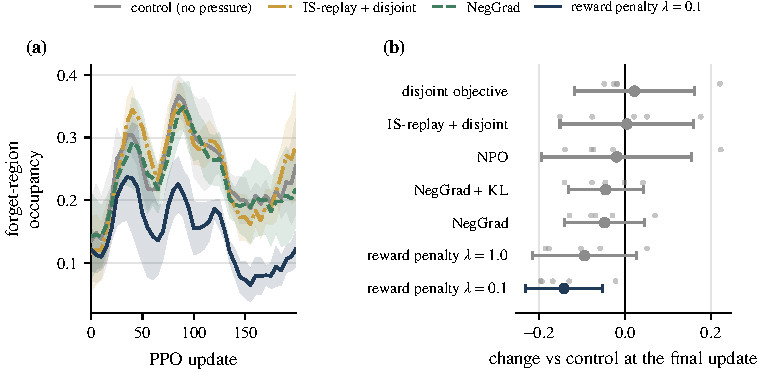
\includegraphics[width=\textwidth]{figures/fig_control.pdf}
\caption{\textbf{(a)} Forget-region occupancy during online unlearning, mean over five seeds with a $95\%$ CI band. The control rises with the others, because occupancy tracks task competence. \textbf{(b)} Change against the control at the final update, paired by seed, with $95\%$ intervals. Small dots are seeds.}
\label{fig:control}\end{figure}
\begin{table}[h]\centering\small
\caption{Final forget-region occupancy and return against the no-pressure control, paired by seed. $p$: paired $t$-test, uncorrected. $p_{\mathrm{Bonf}}$: multiplied by seven.}
\label{tab:comparison}
\begin{tabular}{@{}lccccc@{}}\toprule
Method & Seeds & $\Delta$ occupancy & $p$ & $p_{\mathrm{Bonf}}$ & $\Delta$ return \\ \midrule
disjoint objective & 5 & $+0.071$ & 0.319 & 1.00 & $-0.059$ \\
IS-replay + disjoint objective & 5 & $+0.066$ & 0.227 & 1.00 & $-0.090$ \\
NPO & 5 & $+0.035$ & 0.654 & 1.00 & $+0.046$ \\
NegGrad + KL anchor & 5 & $-0.007$ & 0.796 & 1.00 & $+0.015$ \\
NegGrad & 5 & $-0.020$ & 0.639 & 1.00 & $+0.016$ \\
reward penalty $\lambda=1.0$ & 5 & $-0.074$ & 0.221 & 1.00 & $-0.221$ \\
reward penalty $\lambda=0.1$ & 5 & $-0.113$ & 0.044 & 0.31 & $+0.012$ \\
\bottomrule\end{tabular}\end{table}

\section{Label scope: per-arm results}
\label{app:drift}

Table~\ref{tab:drift} gives the numbers behind Figure~\ref{fig:drift}. Agreement is measured on 4{,}000 states visited by each seed's baseline, with action sampling seeded so that the state set is identical across arms. Occupancy is the fraction of steps in the forget region over 16 evaluation episodes after the last update. $p$ values are paired $t$-tests over the fifteen seeds: for agreement, against the other-scope arm, and for occupancy, against zero.

\begin{table}[h]\centering\small
\caption{Each arm against the \texttt{matching\_steps} run on the same seed (mean, with standard deviation over seeds).}
\label{tab:drift}
\begin{tabular}{@{}llccccc@{}}\toprule
Domain & Arm & Labels changed & Agreement & $p$ & $\Delta$ occupancy & $p$ \\ \midrule
FourRooms & other scope & 20.0\% & 0.537 (0.062) & -- & $+0.046$ (0.074) & 0.030 \\
 & 1\% flips & 1\% & 0.601 (0.069) & 0.003 & $+0.019$ (0.064) & 0.263 \\
 & 10\% flips & 10\% & 0.591 (0.067) & 0.008 & $0.000$ (0.057) & 0.984 \\
 & baseline & -- & 0.544 (0.053) & -- & -- & -- \\
\midrule
CartPole & other scope & 32.6\% & 0.783 (0.147) & -- & $+0.023$ (0.351) & 0.805 \\
 & 1\% flips & 1\% & 0.746 (0.185) & 0.518 & $-0.066$ (0.244) & 0.310 \\
 & baseline & -- & 0.801 (0.141) & -- & -- & -- \\
\bottomrule\end{tabular}\end{table}

The label change is measured on one 2{,}048-step rollout of each seed's baseline, split into episodes as in training, and ranges over seeds from 11.2\% to 34.4\% in FourRooms and from 3.2\% to 72.5\% in CartPole. Compared directly with the 10\% control, the other scope's occupancy shift is larger by 0.046 ($p=0.06$).



\end{document}
